\documentclass[tikz,border=4pt]{standalone}
\usepackage{ctex}
\usepackage{amsmath}
\usetikzlibrary{arrows.meta}

% p8-03a: 待定系数法——两点确定一条直线示意图
% 点(1,3)和(-1,-1)确定直线 y=2x+1
\begin{document}
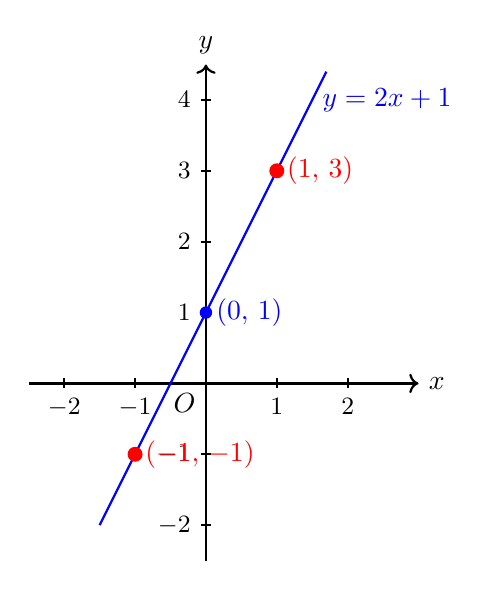
\begin{tikzpicture}[scale=0.9, thick]
  % 坐标轴
  \draw[->] (-2.5,0) -- (3.0,0) node[right] {$x$};
  \draw[->] (0,-2.5) -- (0,4.5) node[above] {$y$};
  \node[below left] at (0,0) {$O$};

  % 刻度
  \foreach \x in {-2,-1,1,2} {
    \draw (\x, 2pt) -- (\x, -2pt) node[below] {\small$\x$};
  }
  \foreach \y in {-2,-1,1,2,3,4} {
    \draw (2pt,\y) -- (-2pt,\y) node[left] {\small$\y$};
  }

  % 直线 y = 2x + 1
  \draw[blue, thick] (-1.5,-2.0) -- (1.7, 4.4);
  \node[right, blue] at (1.5, 4.0) {$y=2x+1$};

  % 两个已知点
  \fill[red] (1,3) circle (3pt);
  \node[right, red] at (1,3) {$(1,\,3)$};

  \fill[red] (-1,-1) circle (3pt);
  \node[right, red] at (-1,-1) {$(-1,\,-1)$};

  % 纵截距
  \fill[blue] (0,1) circle (2.5pt);
  \node[right, blue] at (0,1) {$(0,\,1)$};
\end{tikzpicture}
\end{document}
